%%%%%%%%%%%%%%%%%%%%%%%%%%%%%%%%%%%%%%%%%
% baposter Landscape Poster
% LaTeX Template
% Version 1.0 (11/06/13)
%
% baposter Class Created by:
% Brian Amberg (baposter@brian-amberg.de)
%
% This template has been downloaded from:
% http://www.LaTeXTemplates.com
%
% License:
% CC BY-NC-SA 3.0 (http://creativecommons.org/licenses/by-nc-sa/3.0/)
%
%%%%%%%%%%%%%%%%%%%%%%%%%%%%%%%%%%%%%%%%%

%----------------------------------------------------------------------------------------
%	PACKAGES AND OTHER DOCUMENT CONFIGURATIONS
%----------------------------------------------------------------------------------------

\documentclass[portrait,a0paper,fontscale=0.285]{baposter} % Adjust the font scale/size here

\frenchspacing

\usepackage{graphicx} % Required for including images
\graphicspath{{figures/}} % Directory in which figures are stored

\usepackage{amsmath} % For typesetting math
\usepackage{amssymb} % Adds new symbols to be used in math mode

\usepackage{booktabs} % Top and bottom rules for tables
\usepackage{enumitem} % Used to reduce itemize/enumerate spacing
\usepackage{palatino} % Use the Palatino font
\usepackage[font=small,labelfont=bf]{caption} % Required for specifying captions to tables and figures

\usepackage{multicol} % Required for multiple columns
\setlength{\columnsep}{1.5em} % Slightly increase the space between columns
\setlength{\columnseprule}{0mm} % No horizontal rule between columns

\usepackage{tikz} % Required for flow chart
\usetikzlibrary{shapes,arrows} % Tikz libraries required for the flow chart in the template

\usepackage{epstopdf}

\newcommand{\compresslist}{ % Define a command to reduce spacing within itemize/enumerate environments, this is used right after \begin{itemize} or \begin{enumerate}
\setlength{\itemsep}{1pt}
\setlength{\parskip}{0pt}
\setlength{\parsep}{0pt}
}

\definecolor{lightblue}{rgb}{0.145,0.6666,1} % Defines the color used for content box headers

\definecolor{ourred}{rgb}{0.9,0.0,0.0}

\begin{document}

\begin{poster}
{
headerborder=closed, % Adds a border around the header of content boxes
colspacing=1em, % Column spacing
bgColorOne=white, % Background color for the gradient on the left side of the poster
bgColorTwo=white, % Background color for the gradient on the right side of the poster
borderColor=lightblue, % Border color
headerColorOne=black, % Background color for the header in the content boxes (left side)
headerColorTwo=lightblue, % Background color for the header in the content boxes (right side)
headerFontColor=white, % Text color for the header text in the content boxes
boxColorOne=white, % Background color of the content boxes
textborder=roundedleft, % Format of the border around content boxes, can be: none, bars, coils, triangles, rectangle, rounded, roundedsmall, roundedright or faded
eyecatcher=true, % Set to false for ignoring the left logo in the title and move the title left
headerheight=0.1\textheight, % Height of the header
headershape=roundedright, % Specify the rounded corner in the content box headers, can be: rectangle, small-rounded, roundedright, roundedleft or rounded
headerfont=\Large\bf\textsc, % Large, bold and sans serif font in the headers of content boxes
%textfont={\setlength{\parindent}{1.5em}}, % Uncomment for paragraph indentation
linewidth=2pt % Width of the border lines around content boxes
}
%----------------------------------------------------------------------------------------
%	TITLE SECTION 
%----------------------------------------------------------------------------------------
%
{
\includegraphics[height=8.6em]{leidenland.pdf}} % First university/lab logo on the left
{\bf\textsc{\textcolor{ourred}{Aspects \begin{LARGE}of the cooperative card game\end{LARGE} Hanabi}}\vspace{0.3em}} % Poster title
{\textsc{\begin{large}Steven Student\end{large} \begin{small}(supervized by Bert E. Geleider)\end{small}\\ \begin{small}Leiden Institute of Advanced Computer Science\end{small}\\[0.5mm]}\begin{footnotesize}\texttt{s.tudent@liacs.leidenuniv.nl}\end{footnotesize}} % Author names and institution

%----------------------------------------------------------------------------------------
%	OVERVIEW
%----------------------------------------------------------------------------------------

\headerbox{Overview}{name=objectives,column=0,row=0}{

The game of \textcolor{ourred}{\textsc{Hanabi}} is a cooperative card game in which players together try to obtain the highest possible score. The goal of the game is simple: play out several sequences of cards in the right order. The catch, however, is that the \textbf{players can only see the cards in other player's hands and not their own}; information has to be gathered by a \textbf{system of hints} that reveal partial information.
\vspace{0.5em} % When there are two boxes, some whitespace may need to be added if the one on the right has more content
}

%----------------------------------------------------------------------------------------
%	PLAYABILITY
%----------------------------------------------------------------------------------------

\headerbox{Playability}{name=playability,column=1,row=0,span=2}{

We consider the simplified situation where the players can also
see their own cards. We give a result for the one-player version, with $R=1$: a player must immediately play or discard the newly received card. We consider only one color, but the number of cards of each value can be arbitrary. Hence, the initial stack is now a random sequence of integers in $\{1,\ldots,k\}$.

\vspace{2mm}
The maximum score can be obtained if and only if a subsequence 1--2--\ldots--$k$ exists. The number of ordered sequences with $x_1$ occurrences of the integer~1, 
$x_2$ occurrences of the integer~2, \ldots,
$x_k$ occurrences of the integer~$k$, \emph{without} a
subsequence 1--2--\ldots--$k$, equals

$$
\sum_{\stackrel{\scriptstyle{y\prec\; x}}{|y|\leq k-2}}\!\!\!
\frac
      {(-1)^{|y|}\ (x_1+x_2+\ldots +x_k)!\ (k-|y|-1)^{x_1+x_2+\ldots+x_k-{\scriptstyle{\sum}_{i=1}^k} (y_i\ominus1)}}
      {(y_1\ominus 1)!(y_2\ominus 1)!\ldots(y_k\ominus 1)!(x_1+x_2+\ldots+x_k-\sum_{i=1}^k (y_i\ominus1))!}
$$

Here we denote $t\ominus 1 =\max(t-1,0)$; and $y\prec x$ if
the ordered sequence $y=(y_1,y_2,\ldots,y_k)$ 
satisfies $y_i\leq x_i$ for all $i$; and
$|y|$ is the number of non-zero elements in $y$.
}

%----------------------------------------------------------------------------------------
%	RULES OF THE GAME
%----------------------------------------------------------------------------------------

\headerbox{Rules of the game}{name=method,column=0,below=objectives}{ % This block's bottom aligns with the bottom of the conclusion block

\subsubsection*{Materials and setup}

The ``classic'' game of \textsc{Hanabi} is played with a stack of $N=50$ cards. Every card has one out of $C = 5$ colors and a value between 1 and $k=5$. There are $H = 8$ hint tokens and $E = 3$ error tokens.

At the start of the game, the stack is shuffled and a hand of $R = 4$ or $R = 5$ cards is dealt to each of the $P$ players, $P \in \{2,3,4,5\}$. Now, every player picks up his/her cards in such a way that the other players can see them, but they themselves cannot. The rest of the cards forms the face-down stack. All hint and error tokens are initially available.

\vspace{2mm}
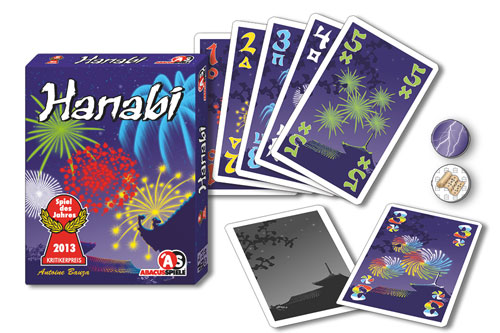
\includegraphics[scale=0.4]{foto.jpg}

\hfill\begin{tiny}Antoine Bauza (2011); published by R \& R Games\end{tiny}

\subsubsection*{Game play}

Every turn, a player chooses one action:
\begin{itemize}
\item Give a \textcolor{ourred}{hint}: expend a hint token to point out all cards of a certain color or value in the hand of one other player.
\item \textcolor{ourred}{Discard} a card: move a card from the hand to the discard pile, regain a hint token and draw a new card from the stack.
\item \textcolor{ourred}{Play} a card: add a card from the hand to its pile on the table (if it fits) or spend an error token; then draw a new card.
\end{itemize}

\subsubsection*{Goal and game end}

The goal of the game is to create $C$ piles of cards going from 1 through $k$ on the table, one of each color. The game ends if either:
\begin{itemize}
\item No error tokens remain: score = 0.
\item All $C$ piles are complete: score = $C \cdot k$.
\item The stack is empty. All players get one more turn; then sum the highest card number in each pile for the score.
\end{itemize} 
\vspace{-1mm}
}

%----------------------------------------------------------------------------------------
%	RULE-BASED-STRATEGY
%----------------------------------------------------------------------------------------

\headerbox{Rule-based strategy}{name=results2,column=1,below=playability}{ % This block's bottom aligns with the bottom of the conclusion block

For the \textcolor{ourred}{rule-based strategy}, every player acts according to the following preset rules:
\begin{enumerate}
\item If there is a card in my hand of which I am ``certain enough'' that it can be played, I play it.
\item Otherwise, if there is a card in my hand of which I am ``certain enough'' that it is useless, I discard it.
\item Otherwise, if there is a hint token available, I give a hint.
\item Otherwise, I discard a card.
\end{enumerate}


%\hspace{2mm}\includegraphics[scale=0.50]{mcgrafiek1a.eps}

%\hspace{2mm}\includegraphics[scale=0.50]{mcgrafiek1d.eps}


Plaatjes, grafieken, \ldots

We show resulting scores for different parameter settings; $P=3$, $R=5$. The highest average score obtained is 15.4.

}

\headerbox{Sample game state}{name=sample,column=1,below=results2,bottomaligned=method}{ % This block's bottom aligns with the bottom of the conclusion block
\begin{footnotesize}
%\vspace{-5mm}
\begin{center}North: $\spadesuit1\ \textcolor{ourred}{\heartsuit3}\ \textcolor{ourred}{\diamondsuit1}\ \spadesuit4\ \clubsuit3$\end{center}

\begin{center}Table: $\textcolor{ourred}{\heartsuit1}\ \textcolor{ourred}{\heartsuit2}$\end{center}

\vspace{-7mm}
\begin{center}$\ \ \ \ \ \clubsuit1$\end{center}


\vspace{-6mm}
West: \hfill East: 

$\spadesuit5\ \clubsuit3\ \textcolor{ourred}{\heartsuit1}\ \clubsuit4\ \clubsuit1$
\hfill $\textcolor{ourred}{\diamondsuit1}\ \textcolor{ourred}{\heartsuit4}\ \spadesuit2\ \spadesuit2\ \spadesuit4$

\begin{center}South (me): $?\ \ ?\ \ ?_2\ ?_2\ ?_{\!\neq2}$\end{center}
\end{footnotesize}

\vspace{-1mm}
South may give North a hint about his/her 1s.

\vspace{3cm}
\begin{center}
Waarom is dit leeg?
\end{center}

}



%----------------------------------------------------------------------------------------
%	MONTE CARLO
%----------------------------------------------------------------------------------------

\headerbox{Monte Carlo strategy}{name=MC,column=2,below=playability,bottomaligned=results2}{ % This block's bottom aligns with the bottom of the conclusion block

The \textcolor{ourred}{Monte Carlo player}
(who does the move with the best average score during random play-outs) uses the following refinements:
\begin{itemize}
\item When playing a card in the Monte Carlo phase, the hand of the current player is shuffled through the deck and a new hand is dealt which is consistent with all hint information obtained so far.
\item During play-outs, the game does not end after 3 errors.
\item The random player does ``reasonable'' moves.
\item Only the score of the next $D$ turns is taken into account to value a play-out.
\end{itemize}

The highest average score obtained is 14.5.
}


%----------------------------------------------------------------------------------------
%	FURTHER RESEARCH
%----------------------------------------------------------------------------------------

\headerbox{Further research}{name=further,column=2,below=MC,bottomaligned=method}{ % This block's bottom aligns with the bottom of the conclusion block

\textbf{Playability:} Try to generalize the given formula for $R > 1$, and find an intuitive proof using the principle of in- and exclusion.

\vspace{2mm}
\textbf{Strategies:} Improve the Monte Carlo player using MCTS or learning methods. Moreover, one can delve deeper in the information truly contained in a given hint (cf. conventions).

\vspace{0.5cm}
\hrule
\vspace{8mm}

Is er nog ergens plek voor Related work?

\vspace{8mm}
Waar staat de onderzoeksvraag?

\vspace{8mm}
Voldoende plaatjes, grafieken, \ldots?

\vspace{8mm}
Deze poster heeft wel erg veel tekst!

\vspace{8mm}
Meer kleur?

\vspace{8mm}
[lastig] En wellicht een conclusie?
}

%----------------------------------------------------------------------------------------

\end{poster}

\end{document}
